%%%%%%%%%%%%%%%%%%%%%%%%%%%%%%%%%%%%%%%%%
% Programming/Coding Assignment
% LaTeX Template
%
% This template has been downloaded from:
% http://www.latextemplates.com
%
% Original author:
% Ted Pavlic (http://www.tedpavlic.com)
%
% Note:
% The \lipsum[#] commands throughout this template generate dummy text
% to fill the template out. These commands should all be removed when 
% writing assignment content.
%
% This template uses a Perl script as an example snippet of code, most other
% languages are also usable. Configure them in the "CODE INCLUSION 
% CONFIGURATION" section.
%
%%%%%%%%%%%%%%%%%%%%%%%%%%%%%%%%%%%%%%%%%

%----------------------------------------------------------------------------------------
%	PACKAGES AND OTHER DOCUMENT CONFIGURATIONS
%----------------------------------------------------------------------------------------

\documentclass{article}
\usepackage{fancyhdr} % Required for custom headers
\usepackage{lastpage} % Required to determine the last page for the footer
\usepackage{extramarks} % Required for headers and footers
\usepackage[usenames,dvipsnames]{color} % Required for custom colors
\usepackage{graphicx} % Required to insert images
\usepackage{caption}
\usepackage{listings} % Required for insertion of code
\usepackage{courier} % Required for the courier font
\usepackage{lipsum} % Used for inserting dummy 'Lorem ipsum' text into the template
\usepackage[colorlinks=true,linkcolor=black,anchorcolor=black,citecolor=black,menucolor=black,runcolor=black,urlcolor=black,bookmarks=true]{hyperref}
\usepackage[table,svgnames]{xcolor}
\usepackage{tabularx}
\usepackage{booktabs}
\usepackage{natbib}
\usepackage{pdfpages}
\usepackage[T1]{fontenc}
\usepackage{amsmath}
\usepackage{fixltx2e}
\usepackage{stackengine}
\usepackage{longtable}
\usepackage{adjustbox}


% Margins
\topmargin=-0.45in
\evensidemargin=0in
\oddsidemargin=0in
\textwidth=6.5in
\textheight=9.0in
\headsep=0.25in

\linespread{1.1} % Line spacing

% Set up the header and footer
\pagestyle{fancy}
\lhead{\hmwkAuthorName} % Top left header
\chead{\hmwkClass\ (\hmwkClassInstructor\ \hmwkClassTime): \hmwkTitle} % Top center head
\rhead{\firstxmark} % Top right header
\lfoot{\lastxmark} % Bottom left footer
\cfoot{} % Bottom center footer
\rfoot{Page\ \thepage\ of\ \protect\pageref{LastPage}} % Bottom right footer
\renewcommand\headrulewidth{0.4pt} % Size of the header rule
\renewcommand\footrulewidth{0.4pt} % Size of the footer rule

\setlength\parindent{0pt} % Removes all indentation from paragraphs

%----------------------------------------------------------------------------------------
%	CODE INCLUSION CONFIGURATION
%----------------------------------------------------------------------------------------

\definecolor{MyDarkGreen}{rgb}{0.0,0.4,0.0} % This is the color used for comments
\lstloadlanguages{Perl} % Load Perl syntax for listings, for a list of other languages supported see: ftp://ftp.tex.ac.uk/tex-archive/macros/latex/contrib/listings/listings.pdf
\lstset{language=Perl, % Use Perl in this example
        frame=single, % Single frame around code
        basicstyle=\small\ttfamily, % Use small true type font
        keywordstyle=[1]\color{Blue}\bf, % Perl functions bold and blue
        keywordstyle=[2]\color{Purple}, % Perl function arguments purple
        keywordstyle=[3]\color{Blue}\underbar, % Custom functions underlined and blue
        identifierstyle=, % Nothing special about identifiers                                         
        commentstyle=\usefont{T1}{pcr}{m}{sl}\color{MyDarkGreen}\small, % Comments small dark green courier font
        stringstyle=\color{Purple}, % Strings are purple
        showstringspaces=false, % Don't put marks in string spaces
        tabsize=5, % 5 spaces per tab
        %
        % Put standard Perl functions not included in the default language here
        morekeywords={rand},
        %
        % Put Perl function parameters here
        morekeywords=[2]{on, off, interp},
        %
        % Put user defined functions here
        morekeywords=[3]{test},
       	%
        morecomment=[l][\color{Blue}]{...}, % Line continuation (...) like blue comment
        numbers=left, % Line numbers on left
        firstnumber=1, % Line numbers start with line 1
        numberstyle=\tiny\color{Blue}, % Line numbers are blue and small
        stepnumber=5 % Line numbers go in steps of 5
}

% Creates a new command to include a perl script, the first parameter is the filename of the script (without .pl), the second parameter is the caption




%----------------------------------------------------------------------------------------
%	DOCUMENT STRUCTURE COMMANDS
%	Skip this unless you know what you're doing
%----------------------------------------------------------------------------------------

% Header and footer for when a page split occurs within a problem environment
\newcommand{\enterProblemHeader}[1]{
\nobreak\extramarks{#1}{#1 continued on next page\ldots}\nobreak
\nobreak\extramarks{#1 (continued)}{#1 continued on next page\ldots}\nobreak
}

% Header and footer for when a page split occurs between problem environments
\newcommand{\exitProblemHeader}[1]{
\nobreak\extramarks{#1 (continued)}{#1 continued on next page\ldots}\nobreak
\nobreak\extramarks{#1}{}\nobreak
}

\setcounter{secnumdepth}{0} % Removes default section numbers
\newcounter{homeworkProblemCounter} % Creates a counter to keep track of the number of problems

\newcommand{\homeworkProblemName}{}
\newenvironment{homeworkProblem}[1][Problem \arabic{homeworkProblemCounter}]{ % Makes a new environment called homeworkProblem which takes 1 argument (custom name) but the default is "Problem #"
\stepcounter{homeworkProblemCounter} % Increase counter for number of problems
\renewcommand{\homeworkProblemName}{#1} % Assign \homeworkProblemName the name of the problem
\section{\homeworkProblemName} % Make a section in the document with the custom problem count
\enterProblemHeader{\homeworkProblemName} % Header and footer within the environment
}{
\exitProblemHeader{\homeworkProblemName} % Header and footer after the environment
}

\newcommand{\problemAnswer}[1]{ % Defines the problem answer command with the content as the only argument
\noindent\framebox[\columnwidth][c]{\begin{minipage}{0.98\columnwidth}#1\end{minipage}} % Makes the box around the problem answer and puts the content inside
}

\newcommand{\homeworkSectionName}{}
\newenvironment{homeworkSection}[1]{ % New environment for sections within homework problems, takes 1 argument - the name of the section
\renewcommand{\homeworkSectionName}{#1} % Assign \homeworkSectionName to the name of the section from the environment argument
\subsection{\homeworkSectionName} % Make a subsection with the custom name of the subsection
\enterProblemHeader{\homeworkProblemName\ [\homeworkSectionName]} % Header and footer within the environment
}{
\enterProblemHeader{\homeworkProblemName} % Header and footer after the environment
}

%----------------------------------------------------------------------------------------
%	NAME AND CLASS SECTION
%----------------------------------------------------------------------------------------

\newcommand{\hmwkTitle}{A5} % Assignment title
\newcommand{\hmwkDueDate}{Friday,\ December\ 15,\ 2017} % Due date
\newcommand{\hmwkClass}{\ INTRO. TO INFO RETRIEVAL:\ CS 734} % Course/class
\newcommand{\hmwkClassTime}{} % Class/lecture time
\newcommand{\hmwkClassInstructor}{Dr. Nelson} % Teacher/lecturer
\newcommand{\hmwkAuthorName}{Udochukwu Nweke} % Your name

%----------------------------------------------------------------------------------------
%	TITLE PAGE
%----------------------------------------------------------------------------------------

\title{
\vspace{2in}
\textmd{\textbf{\hmwkClass:\ \hmwkTitle}}\\
\normalsize\vspace{0.1in}\small{Due\ on\ \hmwkDueDate}\\
\vspace{0.1in}\large{\textit{\hmwkClassInstructor\ \hmwkClassTime}}
\vspace{3in}
}

\author{\textbf{\hmwkAuthorName}}
\date{} % Insert date here if you want it to appear below your name

%----------------------------------------------------------------------------------------

\begin{document}

\maketitle

%----------------------------------------------------------------------------------------
%	TABLE OF CONTENTS
%----------------------------------------------------------------------------------------

%\setcounter{tocdepth}{1} % Uncomment this line if you don't want subsections listed in the ToC

\newpage
\tableofcontents
\newpage

%----------------------------------------------------------------------------------------
%	PROBLEM 1
%----------------------------------------------------------------------------------------

% To have just one problem per page, simply put a \clearpage after each problem

\begin{homeworkProblem}


10.11 Suggest how the maximum and minimum resource ranking scores, $R_{max}$ and $R_{min}$, could be estimated for a given query\\

\textbf{Solution 1:}\\

In a distributed search environment, a meta search engine (main node) broadcasts a query to multiple different search engines (pair nodes). The pair nodes return a result ranking which is merged by the main node.
To select a resource, the main node ranks the pair nodes based on their query likelihood scores for a given query. It then picks the top k nodes which exceed a threshold. After selecting the nodes, a local search is carried out on the nodes and the result is sent to the main node. If the different nodes may have different retrieval models, the ranks from the pair nodes must be normalized before merging to produce a single ranking. The resource ranking score of a  document $S_d$ has to be normalized to get the local ranking of score of the document $S^I_d$ which is the score used to get the final ranking. Figure \ref{fig: resourcenorm} and Figure \ref{fig: docnorm} shows the resource normalization and document normalization respectively.\\


We need to compute $R_{max}$ and $R_{min}$ in order to get the resource normalization scores.\\


\textbf{Estimating $R_{max}$ and $R_{min}$}\\

\textbf{Method 1}\\

$R_{max}$ and $R_{min}$ are the maximum and minimum possible scores for a given query. We can estimate these by finding the highest and lowest scores that the resource ranking algorithm could potentially assign to a node database.  If T in the equation in Figure \ref{fig: estRmaxRmin}  is set to 1, we achieve the maximum score the ranking algorithm can assign to a query - $R_{max}$. If we set T to 0 in Figure \ref{fig: estRmaxRmin}, we get the minimum ranking score a ranking algorithm can assign to a query.\\

\textbf{Method 2}\\

The $R_{max}$ and $R_{min}$ values in Method 1 might be too strict, but $R_{max}$ is often an overestimate in practice. We can also estimate $R_{max}$ and $R_{min}$ by taking finding the maximum ($R_{max}$) and  minimum ($R_{min}$) ranking scores from a corpus statistics: by finding the maximum and minimum ranking scores

\begin{figure}
 \centering
  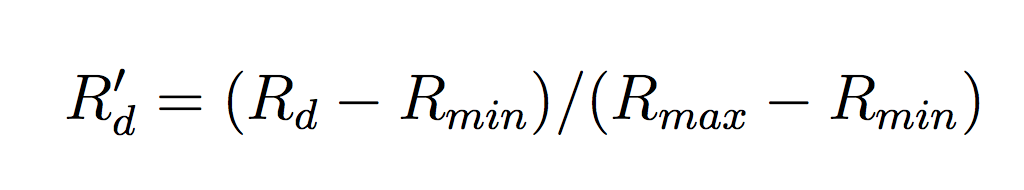
\includegraphics[width=0.5\textwidth]{resourceNormalization.png}
 \caption{Resource Normalization}
 \label{fig: resourcenorm}
 \end{figure}

 \begin{figure}
 \centering
  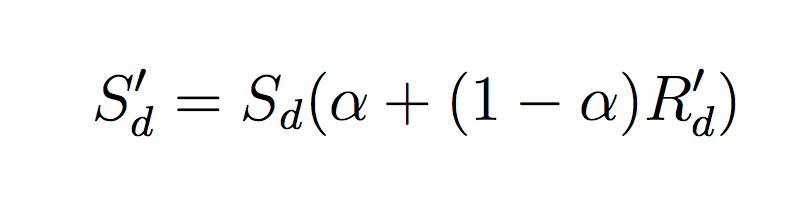
\includegraphics[width=0.5\textwidth]{documentNormalization.png}
 \caption{Document Normalization}
 \label{fig: docnorm}
 \end{figure}

 \begin{figure}
 \centering
  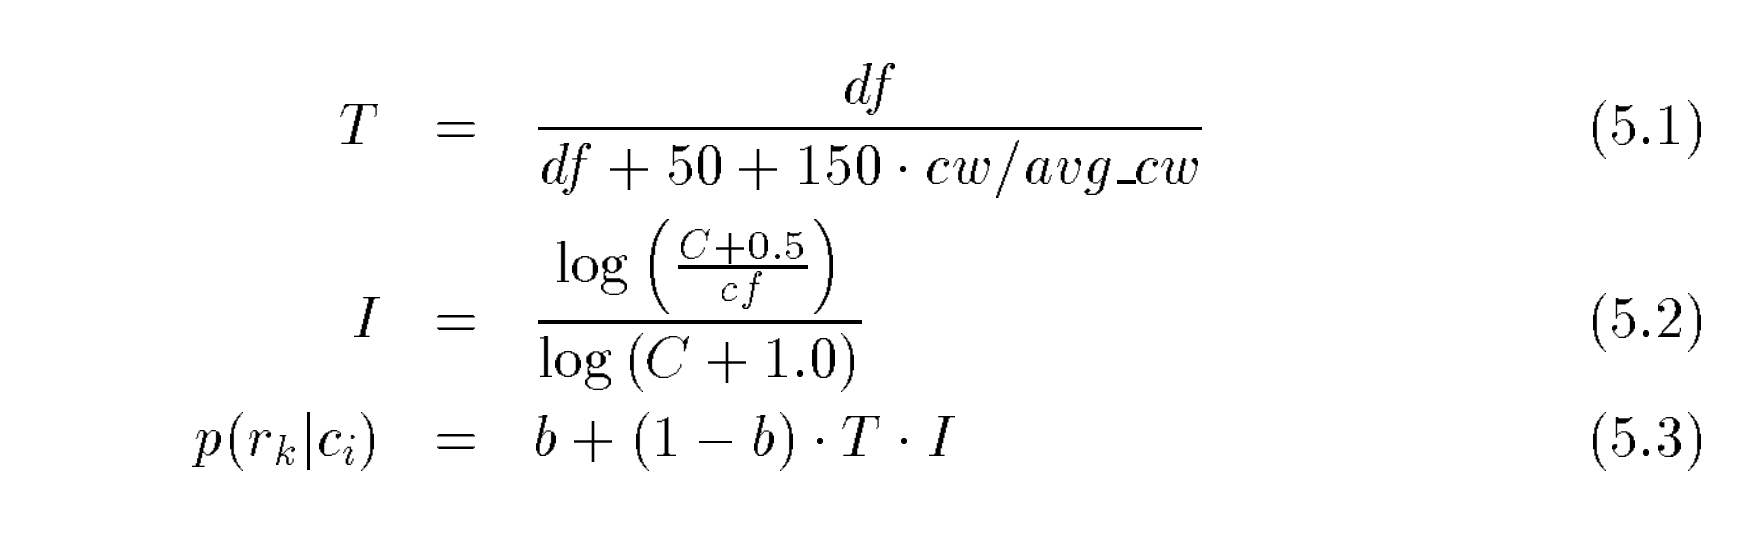
\includegraphics[width=0.5\textwidth]{estRmaxRmin.png}
 \caption{T can be used to estimate $R_{max}$ and $R_{min}$}
 \label{fig: estRmaxRmin}
 \end{figure}




 \end{homeworkProblem}
%----------------------------------------------------------------------------------------
% PROBLEM 2
%----------------------------------------------------------------------------------------


\begin{homeworkProblem}

10.3. Compute five iterations of HITS (see Algorithm 3) and PageRank (see Figure
4.11) on the graph in Figure 10.3. Discuss how the PageRank scores compare
to the hub and authority scores produced by HITS.\\


\textbf{Solution 2:}\\

\lstinputlisting[caption=Five Iterations for HITS and PageRank Code Snippet, language=python]{10.3.py}

I used the python library networkx to apply the HITS and PageRank algorithms to the graphs in Figure \ref{fig: originalgraph}.\\


For both algorithms, the computation did not converge after 5 iterations, so I printed the scores at 5 iterations by modifying the networkx HITS (\textit{hits\_alg.py}) and PageRank (\textit{pagerank\_al.py}) in order to see the scores at 5 iterations. The HITS algotihm converged after 17 iterations while the PageRank algorithm converged after 14 iterations. The result is in Figure \ref{fig: hitandprank}\\


The ranking results of the HITS authority score is the same as the PageRank score. For example, the HITS algorithm ranks the nodes accordingly from highest authority score to lowest authority score:\\
4, 2, 1, (3,5,6,7 - tied)\\
Compared to the PageRank order from highest page rank to lowest:\\
4, 2, 1, (3, 5, 6, 7 - tied)\\

The PageRank algorithm gives an initial rank to nodes without incoming links. This is why the isolated node 7 has the same page rank as nodes 3, 5, and 6 because they all do not have any incoming links. However, the HITS algorithm distinguishes between the isolated node 7 and non isolated nodes 3, 5, and 6.


\begin{figure}
 \centering
  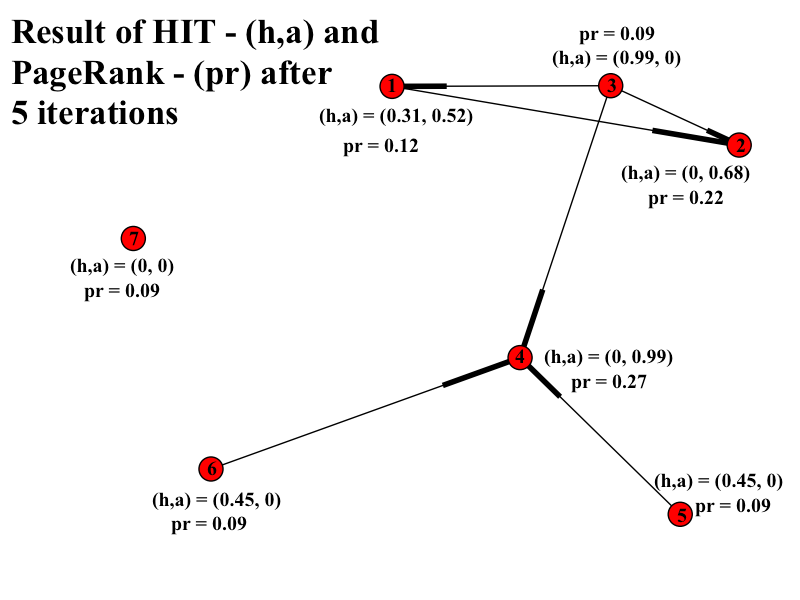
\includegraphics[width=0.5\textwidth]{HITS-PageRankResult.png}
 \caption{HIT and PageRank After 5 iterations}
 \label{fig: hitandprank}
 \end{figure}


 \begin{figure}
 \centering
  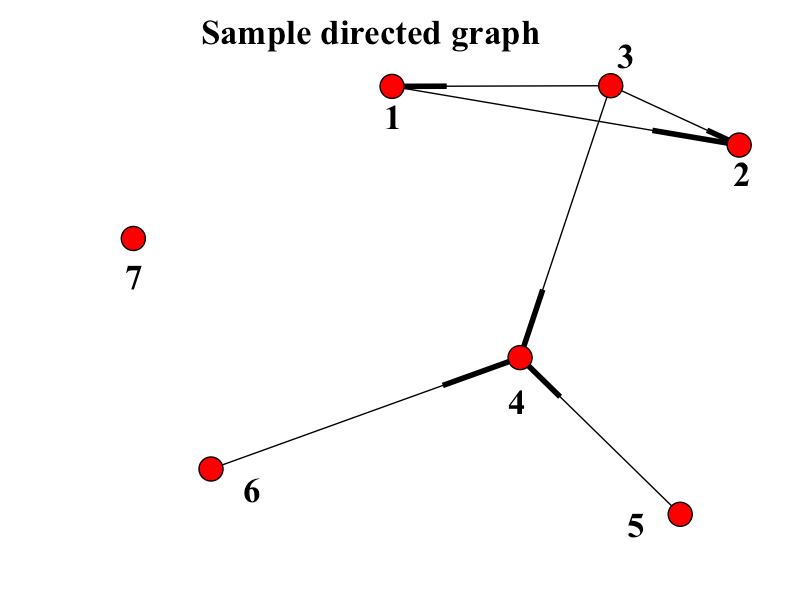
\includegraphics[width=0.5\textwidth]{originalGraph.png}
 \caption{Original Graph}
 \label{fig: originalgraph}
 \end{figure}





\end{homeworkProblem}

%----------------------------------------------------------------------------------------
% PROBLEM 3
%----------------------------------------------------------------------------------------


\begin{homeworkProblem}


10.5. Find a community-based question answering site on the Web and ask two
questions, one that is low-quality and one that is high-quality. Describe the answer
quality of each question.\\

\textbf{Solution 3:}\\

The community-based question and answering system  I used is to ask a high quality ``yahoo question and answer forum''.\\ 
The high quality questuion I ask is :'' How long does it take to get comfortable coding in any programming language?''\\

Observation\\ 

I received answers to this question in a couple of hours. But I received about five informative answers. I was even given some tips and books on how to start and get comfortable with programming. The question and the number of answers is in Figure \ref{fig: hiquality}\\

For my low quality question, I asked: ``What is your favorite bible traanslation?''. I asked this question in \url{https://christianity.stackexchange.com/} and it did not return any answer but it has viewed. After sometime, it was deleted. \\
\\
This is a low quality question because it is a subjective question where every answer is valid. There is no wrong answer.\\


Observation: My observation is that high quality questions receive high quality answers. It might take some time, but the answers are relevant to the questions. Low quality questions on the other hand receive low quality or no answers. They might be viewed sometimes more than the high qulity questions but they are either flagged and possibly removed, depending on how low of a quality they are.\\

\begin{figure}
 \centering
  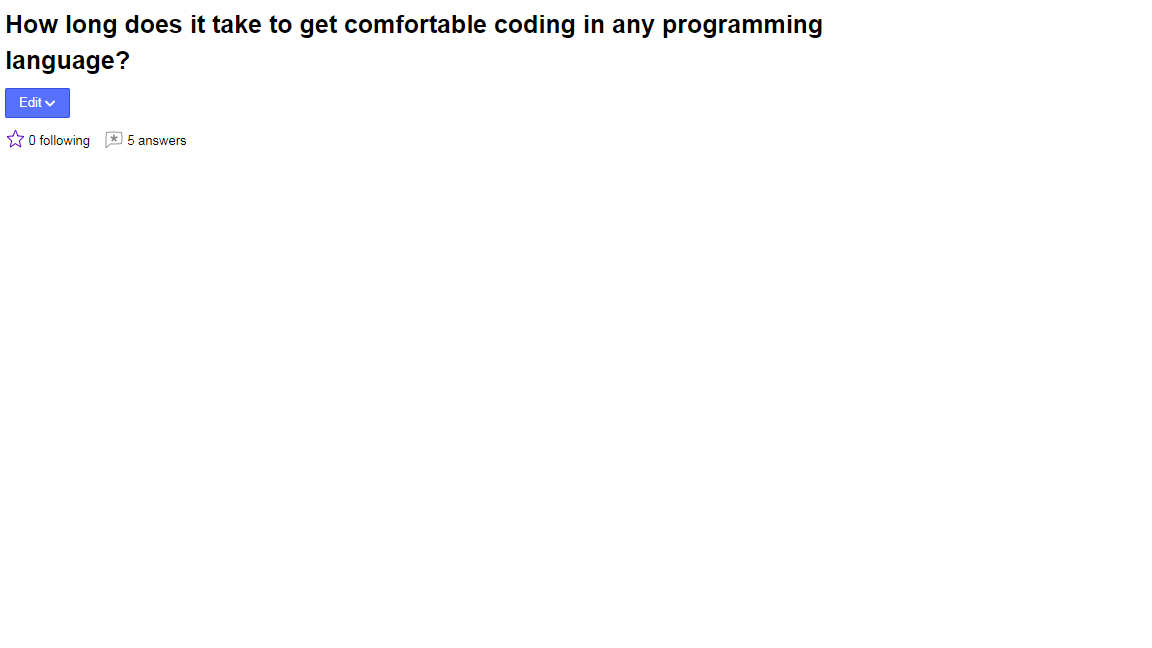
\includegraphics[width=0.5\textwidth]{hquestion.png}
 \caption{High Quality Question}
 \label{fig: hiquality}
 \end{figure}





\end{homeworkProblem}

%----------------------------------------------------------------------------------------
% PROBLEM 4
%----------------------------------------------------------------------------------------

\begin{homeworkProblem}

10.6. Find two examples of document filtering systems on the Web. How do they
build a profile for your information need? Is the system static or adaptive?\\

\textbf{Solution 4:}\\
The document filtering systems:\\
\begin{enumerate}
  \item Amazon
  \item Netflix
\end{enumerate}


Figure\ref{fig: onevsone} is an image of a banner stand I purchased from amazon. After I purchased the banner stand, I have not stopped receiving recommendations from amazon for similair banner stands. Figure\ref{fig: recomen} is an example of the variety of banner stands amazon has been recommending and they are similar to the one I bought. I also have been receiving other items that are not similar to the item I purchase. Some of them are not banner stand. They were purchased from users that also purchased the same banner stand I did. \\

Amazon builds their profile based on products that users purchase. They use this profile to recommended products to users based on similar purchase. This system is adaptive.\\

Just like amazon, Neftlix also uses the same system(adaptive system) to recommend movies to users. When a user sees a movie on Netflix, similar movies are recommended to the user. The user also receives other recommendations based on similar movies that were seen by other users.

 \begin{figure}
 \centering
  
\includegraphics[width=0.5\textwidth]{purchased.png}
 \caption{Purchased Item}
 \label{fig: onevsone}
 \end{figure}

 \begin{figure}
 \centering
  
\includegraphics[width=0.5\textwidth]{recommended.png}
 \caption{Similar items recommended}
 \label{fig: recomen}
 \end{figure}

 \begin{figure}
 \centering
  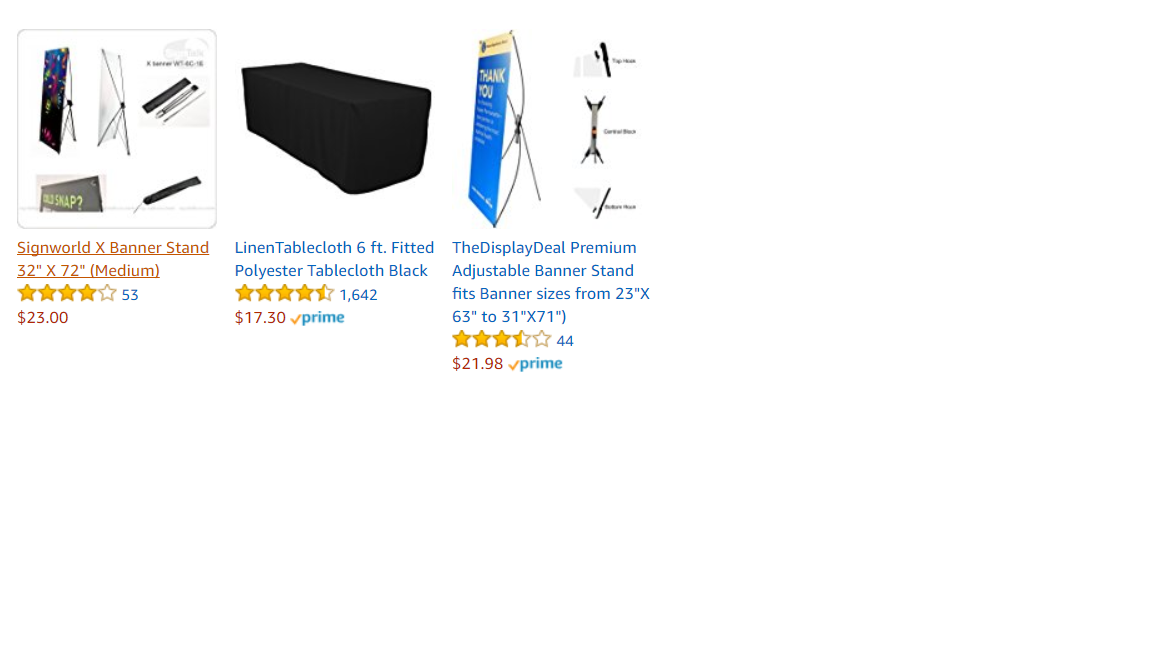
\includegraphics[width=0.5\textwidth]{frequently.png}
 \caption{Dffierent items recommended}
 \label{fig: onevsall}
 \end{figure}



\end{homeworkProblem}
%----------------------------------------------------------------------------------------
% PROBLEM 5
%----------------------------------------------------------------------------------------

\begin{homeworkProblem}

Extra Credit: Wiki Small collection, 8 points extra credit:\\
download the wikipedia.org page URIs from the live web.\\
summarize the HTTP status codes returned-- all 200?  Redirections? 404s?  do we still have 6043 documents?  or have their been splits \&  merges (see also: wikipedia disambiguation pages)?  (1 pt)\\
compare and contrast the in- and out-links from this collection. the number, the domains linked to, the HTTP status of the non-wikipedia links in the article (i.e., are they 200, 404, or something else?). (1 pt)\\
compare the least and most popular articles (in terms of in-links) in the 2008 snapshot vs. the least and most popular articles in your 2017 snapshot. (1 pt)\\
compare and contrast the anchor text for the articles in the collection: are we gaining or losing terms? (1 pt)\\
compare and contrast the sizes of the same pages (i.e., 2008 vs. 2017) in: (2 pts)\\
- bytes\\
- total terms\\
- total unique terms\\
  for all of the pages (i.e., treat each collection as a single unit), compare the 2008 vs. 2017 snapshots in: (2 pts)\\
- bytes\\
- total terms\\
- total unique terms\\

\textbf{Solution 5:}\\

To Download the HTML pages and Get disambiguation pages I used: 
\begin{enumerate}
\item getStatusCodesStatForURLs(): I extracted the wikipedia address from the filenames. For example, the file ``en/articles/1/8/1/1810\_in\_Australia\_7eb1.html'' points to wikipedia page: ``\url{https://en.wikipedia.org/wiki/1810_in_Australia}''
\item getDisambiguationPages(): I identified disambiguation pages by adding \_(disambiguation) to the URLs that returned 200. If a 200 returned a disambiguation page, it means the page has been split. There were X of these. If the page returned a 404 but a 200 for disambiguation page, it means the page has been merged. There were Y of these
\end{enumerate}

The file: \textit{wiki-url-status-codes.txt} has all the status codes

\begin{table}[h!]
 \centering
 \caption{HTTP status returned}
    \label{tab:status}
    \begin{tabular}{| l | l| }
     \hline

  Status&Url Count\\
 \hline
 200&5614\\
 \hline
 404& 420\\
 \hline
 301t& 9\\
 \hline
 
   \end{tabular}
\end{table}

\begin{table}[h!]
 \centering
 \caption{2008 and 2017 Versions}
    \label{tab:versions}
    \begin{tabular}{| l | l| l| }
     \hline

  &2008 Version&2017 Version\\
 \hline
 Bytes&2008-141069412&2017-75641915\\
 \hline
 Terms& 2008-539321& 2017-6342295\\
 \hline
 Unique terms& 2008-75515& 2017-808140\\
 \hline
 
   \end{tabular}
\end{table}

Bytes:\\

For the 2008 version I checked the size the text data utf8len(), the size on disk was 162,556,332, but the corpus folder also had other content.
countBytesLive(): For the 2017 version I made http head request and accumulated the content-length:\\ 
I used sklearn CountVectorizer to create a dictionary with key as the term in the collection and value as the frequency of occurrence in the corpus. See Table \ref{tab:versions} for the number of unique terms and bytes.
I believe the 2008 version is larger because the collection was modified: some of the fields were changed. For example URLs where rewritten, this may have inflated the collection size




\end{homeworkProblem}
%----------------------------------------------------------------------------------------
% PROBLEM 6
%----------------------------------------------------------------------------------------

\begin{homeworkProblem}
11.5. How many papers dealing with term dependency can you find in the SIGIR
proceedings since 2000? List their citations\\

\textbf{Solution 6:}\\

\begin{center}
  \begin{longtable}{|*2{p{3.5cm}| }}
  \hline

  \textbf{Paper} & \textbf{Citations} \\ \hline 
 Two-stage query segmentation for information retrieval&49\\
 \hline
 Capturing term dependencies using a language model based on sentence trees& 94\\
 \hline
 A comparison of retrieval models using term dependencies& 22\\
 \hline
 Learning concept importance using a weighted dependence model& 157\\
 \hline
 Automatic P hrase Indexing for Document Retrieval: An Examination of Syntactic and Non-Syntactic Methods&169\\
 \hline
 [PDF] Capturing term dependencies using a sentence tree based language model& 20\\
 \hline
 Looking inside the box: Context-sensitive translation for cross-language information retrieval& 16\\
 \hline
 Exploring evidence aggregation methods and external expansion sources for medical record search& 16\\
 \hline
 An effective approach to verbose queries using a limited dependencies language model& 19\\
 \hline
  Modeling higher-order term dependencies in information retrieval using query hypergraphs& 54\\
 \hline
  A quasi-synchronous dependence model for information retrievall& 35\\
 \hline
  Modelling term dependence with copulas& 8\\
 \hline
  Parameterized concept weighting in verbose queries& 100\\
 \hline
  Modeling term dependencies with quantum language models for IR& 21\\
 \hline
  The role of knowledge in conceptual retrieval: a study in the domain of clinical medicine& 73\\
 \hline
  Learning to reweight terms with distributed representations& 35\\
 \hline
  [HTML] A dimensional retrieval model for integrating semantics and statistical evidence in context for genomics literature search& 39\\
 \hline
  Word embedding based generalized language model for information retrieval& 22\\
 \hline
[PDF] Weighted Dependence Model," Proceedings of the Third ACM International Conference on Web Search and Data Mining (WSDM 2010). 31 citations.• …& 22\\
 \hline


 
   \end{longtable}
  \end{center}

\end{homeworkProblem}

\nocite{*}
\bibliographystyle{plain}
\bibliography{A5Ref}

\end{document}
